%Talk given virtually for MCM 2021 on special session on QMC software
\documentclass[11pt,compress,xcolor={usenames,dvipsnames},aspectratio=169]{beamer}
%\documentclass[xcolor={usenames,dvipsnames},aspectratio=169]{beamer} %slides and 
%notes
\usepackage{amsmath,
	amssymb,
	datetime,
	mathtools,
	bbm,
	%mathabx,
	array,
	booktabs,
	xspace,
	multirow,
	calc,
	colortbl,
	siunitx,
 	graphicx}
\usepackage[usenames]{xcolor}
\usepackage[giveninits=false,backend=biber,style=nature, maxcitenames =10, mincitenames=9,mincrossrefs=10]{biblatex}
\addbibresource{FJHown23.bib}
\addbibresource{FJH23.bib}
\usepackage{newpxtext}
\usepackage[euler-digits,euler-hat-accent]{eulervm}
\usepackage{media9}
\usepackage[autolinebreaks]{mcode}
\usepackage[tikz]{mdframed}
\usepackage{multicol}


\usetheme{FJHSlimNoFoot169}
\setlength{\parskip}{2ex}
\setlength{\arraycolsep}{0.5ex}

\DeclareMathOperator{\sol}{SOL}
\DeclareMathOperator{\app}{APP}
\DeclareMathOperator{\alg}{ALG}
\DeclareMathOperator{\ACQ}{ACQ}
\DeclareMathOperator{\ERR}{ERR}
\DeclareMathOperator{\COST}{COST}
\DeclareMathOperator{\COMP}{COMP}
\newcommand{\dataN}{\bigl(\hf(\vk_i)\bigr)_{i=1}^n}
\newcommand{\dataNj}{\bigl(\hf(\vk_i)\bigr)_{i=1}^{n_j}}
\newcommand{\dataNjd}{\bigl(\hf(\vk_i)\bigr)_{i=1}^{n_{j^\dagger}}}
\newcommand{\ERRN}{\ERR\bigl(\dataN,n\bigr)}

\newcommand{\Sapp}{S_{\textup{app}}}
\newcommand{\LambdaStd}{\Lambda^{\textup{std}}}
\newcommand{\LambdaSer}{\Lambda^{\textup{ser}}}
\newcommand{\LambdaAll}{\Lambda^{\textup{all}}}
\newcommand{\oton}{1\!:\!n}
\newcommand{\talert}[1]{\alert{\text{#1}}}
\DeclareMathOperator{\init}{init}
\DeclareMathOperator{\GP}{\cg\cp}
\newcommand{\MLE}{\textup{EB}}
\newcommand{\mCtheta}{{\mathsf{C}_{\vtheta}}}
\newcommand{\mCInv}{\mathsf{C}^{-1}}

%\DeclareMathOperator{\app}{app}

\providecommand{\HickernellFJ}{H.\xspace}


\iffalse
Quasi-Monte Carlo (qMC) theory has developed over than six decades.  Computer implementations of quasi-Monte Carlo algorithms have followed behind.  With practitioners seeking ways to speed up their Monte Carlo calculations, and theorists eager to see qMC expand into new application areas, we need qMC software that is reliable, efficient, accessible, comprehensive, and easy-to-use.  This talk describes the progress that has been made so far by various groups and what challenges lie ahead.
\fi

\renewcommand{\OffTitleLength}{-7ex}
\setlength{\FJHThankYouMessageOffset}{-8ex}
\title{Advances and Challenges in Quasi-Monte Carlo Software}
\author[]{Fred J. Hickernell}
\institute{Department of Applied Mathematics \&
	Center for Interdisciplinary Scientific Computation \\  Illinois Institute of Technology \quad
	\href{mailto:hickernell@iit.edu}{\url{hickernell@iit.edu}} \quad
	\href{http://mypages.iit.edu/~hickernell}{\url{mypages.iit.edu/~hickernell}}}

\thanksnote{with Sou-Cheng Choi, Mike McCourt, Jagadeeswaran Rathinavel, Aleksei Sorokin \\ 
and the rest of the QMCPy team \\[2ex]
	Thanks to the organizers, especially during these unusual times \\
	Slides at  \href{https://speakerdeck.com/fjhickernell/advances-and-challenges-in-quasi-monte-carlo-software}{\nolinkurl{speakerdeck.com/fjhickernell/advances-and-challenges-in-quasi-monte-carlo-software}}}

\event{MCM 2021}
\date[]{August 17, 2021}

\input FJHDef.tex


\newlength{\figwidth}
\setlength{\figwidth}{0.25\textwidth}

\newlength{\figwidthSmall}
\setlength{\figwidthSmall}{0.2\textwidth}

\newcommand{\financePict}{\href{http://i2.cdn.turner.com/money/dam/assets/130611131918-chicago-board-options-exchange-1024x576.jpg}{\includegraphics[width
		= 3cm]{ProgramsImages/130611131918-chicago-board-options-exchange-1024x576.jpg}}}
	
	\newcommand{\scoop}[1]{\parbox{#1}{
\includegraphics[width=#1]{IceCreamScoop.eps}}\xspace}
	\newcommand{\smallscoop}{\scoop{1cm}}
	\newcommand{\medscoop}{\scoop{1.8cm}}
	\newcommand{\largescoop}{\scoop{3cm}}
	\newcommand{\ICcone}[1]{\parbox{#1}{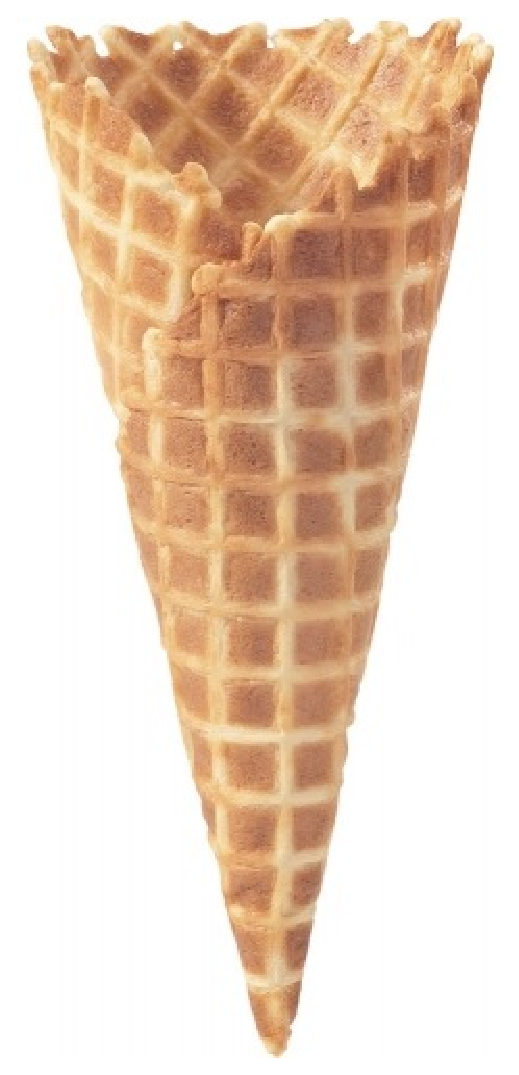
\includegraphics[width=#1,angle=270]{MediumWaffleCone.eps}}\xspace}
	\newcommand{\medcone}{\ICcone{1.2cm}}
	\newcommand{\largercone}{\parbox{2.2cm}{\vspace*{-0.2cm}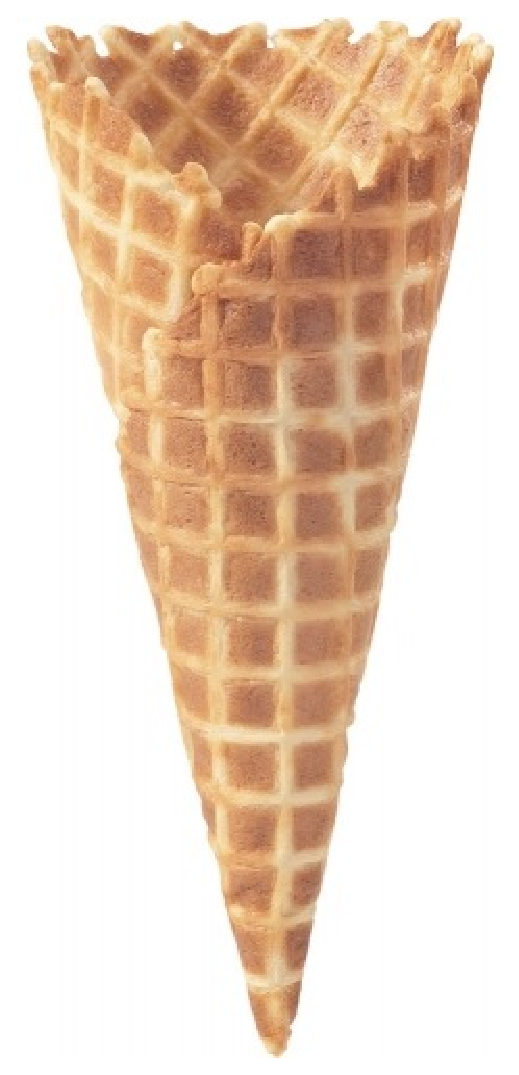
\includegraphics[width=1cm,angle=270]{MediumWaffleCone.eps}}\xspace}
	\newcommand{\largecone}{\ICcone{1.8cm}}
	\newcommand{\smallcone}{\parbox{1.1cm}{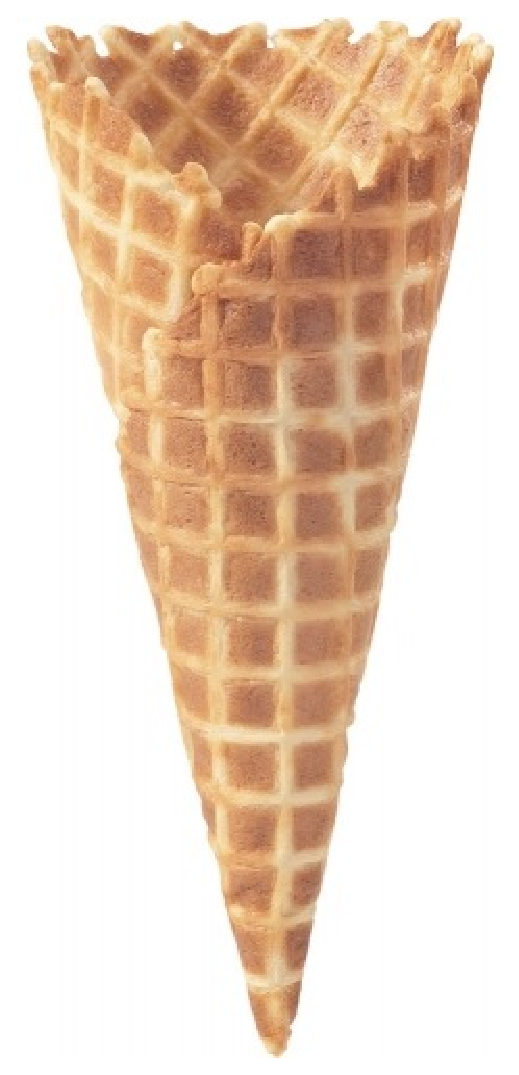
\includegraphics[width=0.5cm,angle=270]{MediumWaffleCone.eps}}\xspace}

	

\newcommand{\northeaststuff}[3]{
	\begin{tikzpicture}[remember picture, overlay]
	\node [shift={(-#1 cm,-#2 cm)}]  at (current page.north east){#3};
	\end{tikzpicture}}


\begin{document}
	\tikzstyle{every picture}+=[remember picture]
	\everymath{\displaystyle}

\frame{\titlepage}

\section{Background}

\begin{frame}{Quasi-Monte Carlo Cubature}
	
	\vspace{-6ex}
	
	\[
	\uncover<3->{\mu :=  \int_{\ct} \alert<4>{g(\vt)} \, \alert<3>{\lambda(\vt) \, \dif \vt} \underbrace{=}_{\alert<3>{\vt = \vT(\vx)}} } \only<1>{\mu :=} 	\underbrace{\int_{[0,1]^d} \alert<4>{f(\vx)} \, \dif \vx}_{\text{integration}} =  \underbrace{\Ex[f(\vX)]}_{\text{expectation}} \approx  \underbrace{\frac 1{\alert<5>{n}} \sum_{i=1}^{\alert<5>{n}} f(\alert<2>{\vX_i})}_{\text{sample mean}} =: \hmu_{\alert<5>{n}}
	\]
	
	\vspace{-3ex}
	
	\begin{description}[<+(1)->]
		\setlength{\itemsep}{0.5cm}
		
		\item[Low Discrepancy Generator] producing $\vX_1, \vX_2, \dots \LDsim \cu[0,1]^d$ 
		
		\item[True Measure] $\lambda$ used to define the original integral, such as Lebesgue or Gaussian, along with the variable transformation (importance sampling)
		
		\item[Integrand] $g$ used to define original integral and the final, transformed integrand, $f(\vx) = g(\vT(\vx))\lambda(\vT(\vx))\abs{\vT'(\vx)}$ (preferably flat)
		
		\item[Stopping Criterion] that determines how large $n$ should be to ensure that $\abs{\mu - \hmu_n} \le \varepsilon$
	\end{description}
\end{frame}

\begin{frame}{Software Landscape}
	\vspace{-3ex}
	{\small 
	
	\renewcommand{\arraystretch}{1.15}
	\begin{tabular}{>{\centering}m{0.47\textwidth}@{\qquad}>{\centering}m{0.47\textwidth}}
		\alert{LD Sequence Generators} & \alert{Multi-Level, Stopping Criteria, Applications}
		\tabularnewline \toprule
		\href{https://www.mathworks.com}{\alert{MATLAB Statistics Toolbox}}---\newline Sobol' and Halton &
		\href{https://people.maths.ox.ac.uk/gilesm/mlmc/}{\alert{Mike Giles}}---Multi-Level (Quasi-)Monte Carlo  in C++, MATLAB, Python, and R
		\tabularnewline
		\href{https://cran.r-project.org/web/packages/qrng/qrng.pdf}{\alert{Marius Hofert \& Christiane Lemieux }}---\texttt{qrng} R package, Sobol' and Halton &
		\href{http://gailgithub.github.io/GAIL_Dev/}{\alert{Guaranteed Automatic Integration Library (GAIL)}}---Stopping criteria  in MATLAB
		\tabularnewline
		\href{http://www.broda.co.uk}{\alert{BRODA, Sergei Kucherenko}---Sobol' in C, MATLAB, and Excel}& 
		\href{https://www.uqlab.com}{\alert{UQLab}}---Framework for Uncertainty Quantification in MATLAB
		\tabularnewline
		\href{http://statweb.stanford.edu/~owen/code/}{\alert{Art Owen}}---randomized Halton in R&
		\multirow{3}{0.47\textwidth}{\centering \href{http://www.openturns.org}{\alert{OpenTURNS}---An Open source initiative for the Treatment of Uncertainties, Risks 'N Statistics in Python}}
		\tabularnewline
		\href{https://github.com/PieterjanRobbe/QMC.jl}{\alert{Pieterjan Robbe}---LD sequences in Julia}
		\tabularnewline
		\href{https://Sci.Py.org/}{\alert{SciPy}}, \href{https://pytorch.org/}{\alert{PyTorch}---Sobol' in Python}
		\tabularnewline
		\alert{Tensorflow}---(Digital) lattices in Python
		\tabularnewline
		\href{https://developer.nvidia.com/curand}{\alert{cuRAND}}---Sobol' in CUDA
	\tabularnewline
		\multicolumn{2}{>{\centering}m{0.96\textwidth}}{\href{http://simul.iro.umontreal.ca}{\alert{Pierre L'Ecuyer}---LatNet Builder and  Stochastic Simulation in C/C++ and Java}}
		\tabularnewline
		\multicolumn{2}{>{\centering}m{0.96\textwidth}}{\href{https://people.cs.kuleuven.be/~dirk.nuyens/}{\alert{Dirk Nuyens}}---Magic Point Shop and QMC4PDE in MATLAB, Python, and C++}
		\tabularnewline
		\multicolumn{2}{>{\centering}m{0.96\textwidth}}{\href{http://people.sc.fsu.edu/~jburkardt/}{\alert{John Burkhardt}}---variety in C++, Fortran, MATLAB, \& Python}
		\tabularnewline
		\multicolumn{2}{>{\centering}m{0.96\textwidth}}{\href{https://qmcsoftware.github.io/QMCSoftware/}{\alert{QMCPy}}---Python package incorporating and connecting the work of different groups}
		\tabularnewline
	\end{tabular}
	
}
	
	\renewcommand{\arraystretch}{1}
	
\end{frame}

\begin{frame}{What We Want}
\begin{multicols}{2}
	\begin{itemize}
		\item QMC in the hands of more users
		
		\item Quality QMC algorithms
		
		\item Platform to compare performance of QMC algorithms
		
		\item Vehicle to explore QMC for new use cases
		
	\end{itemize}
	
	\columnbreak
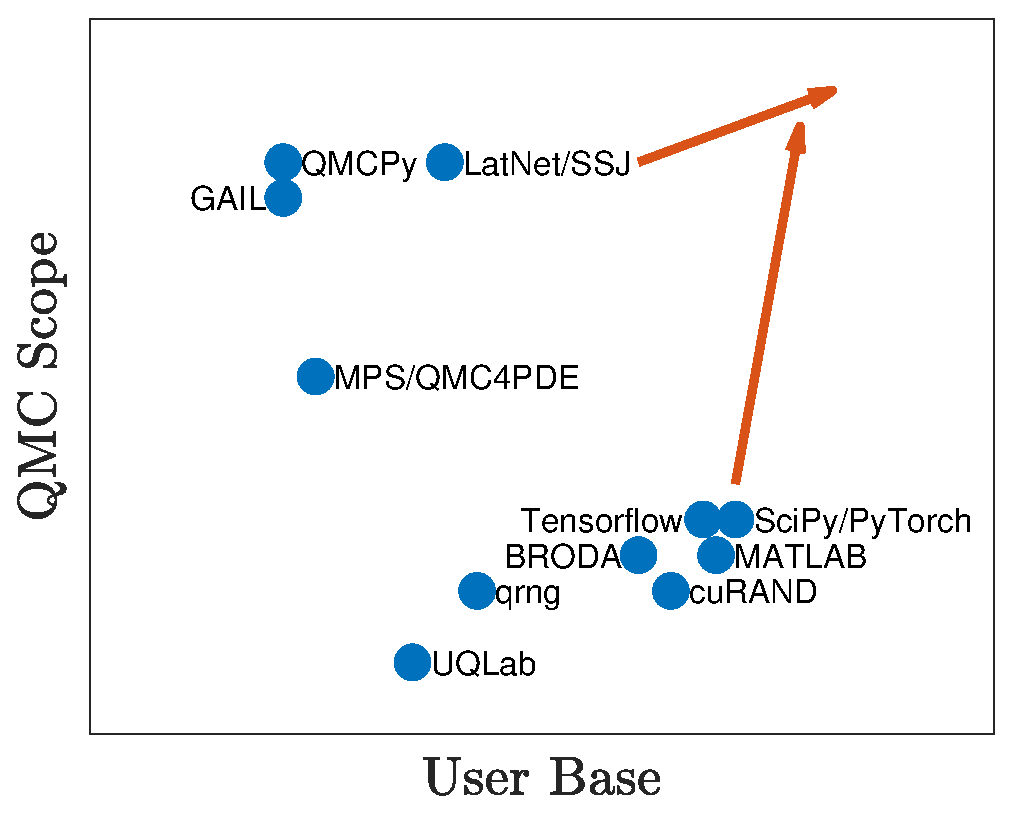
\includegraphics[width = 0.45\textwidth]{QMCSoftwarePlot.eps}	
\end{multicols}

\end{frame}


\section{Low Discrepancy Generators}

\begin{frame}{Low Discrepancy Generators: $\vX_1, \vX_2, \dots \LDsim \cu[0,1]^d$}
\begin{multicols}{2}
{\Large \alert{Recent Advances}}
\begin{itemize}
	\item \href{https://github.com/scipy/scipy/pull/10844}{\alert{Sobol' and Halton into SciPy.}}  Zeroth point included.  Cython for speed.
	
	\item Lattices and digital nets into \alert{Tensorflow}
	
	\item Niederreiter points and other ``bring your own'' generators in QMCPy
	
\end{itemize}

\columnbreak
\uncover<2>{
{\Large \alert{Challenges}}
\begin{itemize}
	\item Need to educate \href{https://arxiv.org/pdf/2008.08051.pdf}{\alert{against}} dropping, thinning, burn-in, power of $10$ sample sizes \cite{Owe22a}
	
	\item \alert{Nested uniform scrambling} of nets \cite{Owe95} not yet widely available
	
	\item \alert{Higher order nets} not widely available
	
	\item \alert{Which} generators are significantly better 
	\begin{itemize}
		\item For which practical problems?
		\item For higher dimensions?
	\end{itemize}

\item Is there a useful hybrid of lattices and digital sequences?
\end{itemize}
}

\end{multicols}
\end{frame}

\section{True Measures}

\begin{frame}{True Measures $\vT: \ct \to [0,1]^d$ }

\vspace{-8ex}
	\[
\int_{\ct} g(\vt) \, \lambda(\vt) \, \dif \vt \underbrace{=}_{\alert{\vt = \vT(\vx)}} \int_{[0,1]^d} f(\vx) \, \dif \vx \qquad \text{\alert{Variable transformations} aka \alert{importance sampling}}
\]

	\begin{multicols}{2}
		{\Large \alert{Recent Advances}}
		\begin{itemize}
			\item QMCPy has defaults for $\vT = \reals^d$ or $[\va,\vb]^d$ based on  the original weight function, and you can choose your own
						
		\end{itemize}
		
		\columnbreak
		
		\uncover<2>{
		{\Large \alert{Challenges}}
		\begin{itemize}
			\item Importance sampling is an art
			
			\item Need for \href{https://statweb.stanford.edu/~owen/pubtalks/AdaptiveISweb.pdf}{\alert{adaptive importance sampling}}
			
			\item Transformations for non-rectangular $\ct$ (simplex, ball, sphere)  not widely available
			
		\end{itemize}
	}
		
	\end{multicols}
\end{frame}

\section{Integrands}

\begin{frame}{Integrands or Use Cases $	\int_{\ct} \alert{g(\vt) \, \lambda(\vt)} \, \dif \vt = \cdots$}
	
	\begin{multicols}{2}
		{\Large \alert{Recent Advances}}
		\begin{itemize}
			\item QMCPy allows you to build your own, and has several examples
			
			\item UQLab and OpenTURNS include LD generators for their use cases
			
			\item Some new use cases such as in Robbe's talk \cite{Vro19a} on system reliability and Ebert's talk combining QMC with algorithmic differentiation
			
		\end{itemize}
		
		\columnbreak
		
		\uncover<2>{
			{\Large \alert{Challenges}}
			\begin{itemize}
				\item Our use cases need refreshing and expanding
				
				\item Hard to swap out different LD generators for important use cases because the use cases do not have a common interface or is not always accessible
				
				\item Need to demonstrate connecting a package that computes the integrand values (such as an open source PDE solver) with the package that does the QMC
				
			\end{itemize}
		}
		
	\end{multicols}
\end{frame}

	
\section{Stopping Criteria}

\begin{frame}{Stopping Criteria, $n = ?$ to Satisfy Error Tolerance}
	
	\begin{multicols}{2}
		{\Large \alert{Recent Advances}}
		\begin{itemize}
			\item QMCPy includes 
			\begin{itemize}
				\item Several kinds of stopping criteria (replications, tracking Fourier coefficients \cite{HicJim16a,JimHic16a}, Bayesian credibility intervals \cite{RatHic19a})
				\item Criteria to ensure that $\abs{\sol - \sol_n} \le   \max(\varepsilon_{\text{a}}, \varepsilon_{\text{r}} \abs{\sol})$, where
				$\sol$ is a function of more than one integral (Bayesian inference, Sobol' indices)
			\end{itemize}
						
		\end{itemize}
		
		\columnbreak
		
		\uncover<2>{
			{\Large \alert{Challenges}}
			\begin{itemize}
				\item Need better stopping criteria for higher order nets (other than replications)
				
				\item Need better stopping criteria for more complex problems, such as parametric integration, density estimation, Markov Chain Monte Carlo
				
			\end{itemize}
		}
		
	\end{multicols}
\end{frame}



\finalthanksnote{These slides are  available at \\  \href{https://speakerdeck.com/fjhickernell/advances-and-challenges-in-quasi-monte-carlo-software}{\nolinkurl{speakerdeck.com/fjhickernell/advances-and-challenges-in-quasi-monte-carlo-software}}}


\thankyouframe

\printbibliography


\end{document}





